\section{Focus of this Report}
A surgery consists of a series of subtasks, some suited for robotized autonomous execution. Prior work in motion planning and control of subtasks for surgical robots include knot tying, suturing and more advanced statistical learning of subtasks from recording surgeon motions \citep{bib:raven_debride,bib:raven_observ}.

This report presents the work on a guaranteed safe end-effector trajectory control. As opposed to the safety control by virtual potential field constraints \citep{bib:dlr_miro}, this work utilizes the barrier certificate method where the robot is physically prevented from entering unsafe areas thereby guaranteeing safety \citep{bib:safety}. A short overview of the controller is given in \autoref{sec:project_overview}.

The algorithm is tested on a first generation da Vinci surgical robot, detached from its surgeon controller console and modified to be controllable by automated processes. An overview of the system is given in \autoref{sec:technical_overview}.


%One should certainly take the risk of patient trauma when an automated surgery is conducted into account. This is seen in Therac-25. 



\subsection{Technical Overview of the Robotic Surgery System}\label{sec:technical_overview}
A simplified overview of the robot controller setup is provided in \autoref{fig:overview}. The setup is physically located at the Control and Automation laboratory at Aalborg University. 

\Autoref{fig:overview} is structured in descending abstraction layers with the highest at the top (i.e. the \gls{ros} - an open source software framework for robots \citep{bib:ros}, see \autoref{app:ros} for further details), which establishes a wireless TCP/IP communication channel receiving all positions from the robot as feedback and produces position control signals to the NI (National Instruments) single board \glspl{rio} which handle all input/output communication with the user. The NI single board \glspl{rio} consist of a primary and a secondary board. The reason for having two \gls{rio} boards is solely the lack of input/outputs on one board.

The \gls{rio} boards direct the control signals to a cascaded controller taking in the position reference from the user and delivering a current control signal to the ESCON motor driver. The velocity and current controllers are implemented in \gls{fpga} based hardware to ensure sufficient controller speed relative to the system \citep{bib:robot_paper}. The ESCON motor driver manage advanced processing and essentially delivers an appropriate PWM signal for the actuators (seven maxon motors) which represent the lowest abstraction layer, located at the bottom of the figure.

The NI single board \glspl{rio} concurrently handle most safety precautions and enabling/disabling movement of the arm itself (see appendix ?? for location of the arm) through solenoids.
\begin{figure}[H]
	\center
		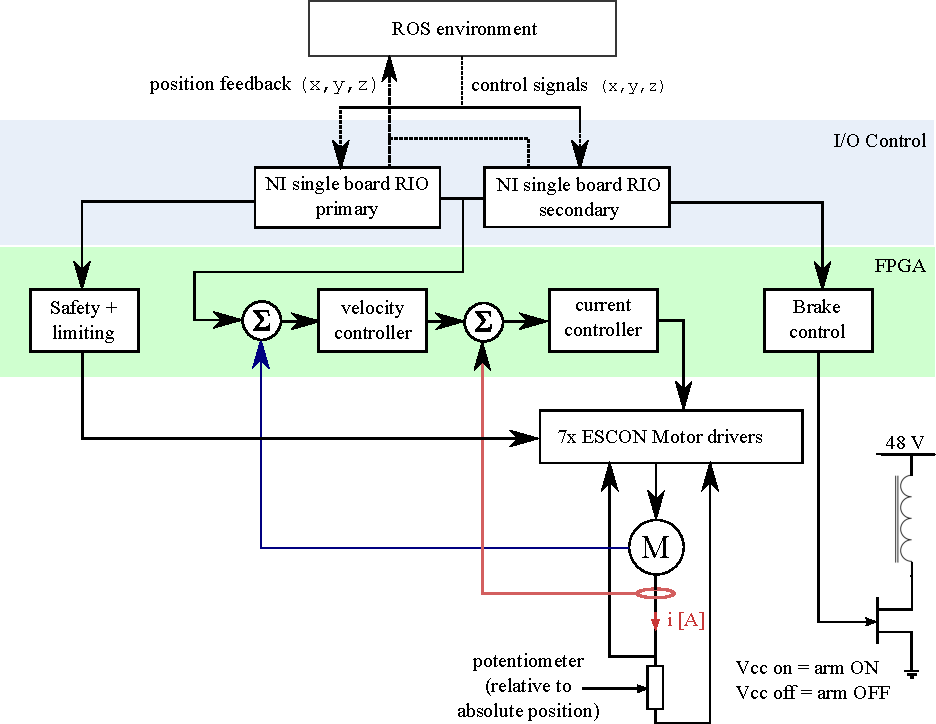
\includegraphics[width=0.95\textwidth]{overview.pdf}	\caption{This is a nice figure. Here illustrated for hand roll master.}
	\label{fig:overview}
\end{figure}
The focus of this thesis is the highest abstraction layer, i.e.the ROS environment. The purpose here primary constitute implementation of:
\begin{itemize}
\item Everything that require heavy processing \citep{bib:robot_paper}.
\item Non real-time processing or tasks with loose timing constraints \citep{bib:robot_paper}.
\end{itemize}
The above pool of stipulations will essentially and practically entail the following main topics of this thesis:
\begin{itemize}
\item All user interaction
\item Positioning control loops
\item Path planning
\end{itemize}
A crucial matter when dealing with those topics within robotic surgeries feature necessary conditions to guarantee the patient safety and to avert patient trauma \citep{bib:safety}.


\subsection{Project Overview}\label{sec:project_overview}
The system consists of the surgical robot arm, which must follow a trajectory on the surface of a beating heart. This means that the setpoint will follow the heart's motion, and the coordinate frame fixed at the setpoint will translate and rotate according to the beating-heart model described in \citep{bib:heart_model,bib:safety}.

The input to the system will be the endpoint of a trajectory, and the ROS software will generate a trajectory and appropriate setpoints for the low-level controllers (which have been designed to be aggressive such that the system will react to small changes in desired position, and hence does not work well with large changes). The trajectory planning must take into account a Lyapunov function for the system, that ensures stability (what would instability mean in this case? would it be oscillations of the arm? the low-level controllers already implement constraints on the position preventing the system to reach its physical limits) and the barrier certificate, which imposes limits that physically cannot be violated by the system (in what way is this much more safe and a better mathematical guarantee of safety than virtual potential fields?), and hence limits the set of possible trajectories. These two functions can be combined in a barrier certificate control function (still need to perceive how), which must be or be connected to the trajectory planning algorithm.

The beating heart (moving setpoints/trajectory) can be seen as a disturbance, or uncontrollable input, and the beating heart model is included in the controller so the setpoint to send to the system should be as if the surface was immobile. The controller then handles both the trajectory planning with avoidance of unsafe areas, and the translation of the trajectory to the instantaneous surface point. The latter should be done by the time periodic transformation matrix (translation and rotation) between the beating heart setpoint coordinate frame, and the instrument end-effector coordinate frame. The setpoints may be given in the absolute (inertial) coordinate frame, and the transformation to end-effector coordinate frame (position and orientation) is given by the sequence of transformation matrices between each joint in the robot arm given in \cite{bib:heart_model}.

In the continuous nonlinear system state space equation
\begin{equation}
\dot{x}=f(x)+g(x)\cdot k(x)
\end{equation}
the function $f(x)$ will hold the dynamics (and kinematics?) of the system, and $k(x)$ is the control input to the system (which implements the barrier certificate and somehow also the Lyapunov controller). Could this mean that $g(x)$ could be the beating heart model, and that $k(x)$ then should include some inverse function of this model in order for the setpoint/reference to be positions on the immobile surface of the heart at time $t_0$?
If the system always moves very slowly, acceleration may be ignored and maybe dyamics could be ignored altogether, only leaving the evolution of kinematics in the function $f(x)$.

It is desired at the end of the project to perform a trajectory following task with the robot arm (not only simulations or visualization through the ROS tool Rviz), and for that a tissue phantom must be procured, which allows for multiple tests with cutting tools. The phantom is desired to be able to imitate the motion of a beating heart, i.e. including a pump or other system allowing the surface to translate and rotate according to the beating heart model given in \citep{bib:heart_model}. This, however, seems to be an obstacle, since phantoms of moving hearts suited for cutting may not exist, or if they do may be too expensive. Alternatively a smaller/simpler phantom could be procured, allowing for attachment of a pump system, but in that case, would we not also have to design a pump system that would make the specific phantom translate as described in the model (but how could we possibly design it to also obtain the exact rotation if it has the wrong size and must be controlled by a simple pump system?)


%Raven-II inverse control process (not primarily to estimate the pose, in which case standard estimation methods like Kalman would be appropriate) is to calculate, give an desired true pose, the input pose to send the control sw to reach the desired true pose (detected pose with vision system assumed to be the true pose), estimate between measurements using updates from forward kinematics \citep{bib:raven_debride}.

%advances in motion planning, control and perception: integrated task and motion planning ofhigh level task planning using state machines, and motion planning for low level planning algorithm  \citep{bib:raven_debride}

%da Vinci Research Kit: learning from demonstrations/by observation. Targets considered form convex regions spherical/linear. \citep{bib:raven_observ}.